\chapter{Sharing-aware thread mapping in STM}\label{chap:sharAwareThreadMap}

This chapter describes two mechanisms to perform sharing-aware thread mapping in STM applications. We start proposing a \emph{static} mechanism~(Section~\ref{sect:staticThreadMap}), i.e., where threads are mapped to cores at the beginning of execution, based on a previous analysis of the sharing behavior of the application. Next, an \emph{online} mechanism is presented~(Section~\ref{sect:onlineThreadMapping}). In an online strategy, the detection of sharing behavior and thread migration is performed based on information gathered during execution.

\section{Static thread mapping}\label{sect:staticThreadMap}

Since the experiments in Chapter~\ref{chap:charact} showed that \texttt{STAMP} applications do not present dynamic sharing behavior, our hypothesis is that a \emph{static} thread mapping mechanism (where threads are mapped to cores at the beginning of execution, and never migrated) is sufficient to improve the performance of \texttt{STAMP} applications. Many tools are available to calculate a thread mapping based on a communication matrix, for instance, \texttt{Scotch}~\cite{Pellegrini:1994}, \texttt{TreeMatch}~\cite{TreeMatch}, \texttt{EagerMap}~\cite{Cruz:2019}  and \texttt{ChoiceMap}~\cite{Soomro:2018}. We opted to use \texttt{TopoMatch}~\cite{TopoMatch} which integrates \texttt{Scotch} and \texttt{TreeMatch} in the same library to deal with any kind of machine topology. \texttt{TopoMatch} uses the \texttt{hwloc} library~\cite{hwloc} to compute the hierarchical topology of the machine. The thread mapping is calculated taking into consideration the machine topology. Hence, the idea is to use the mechanism described in Chapter~\ref{chap:mechanism} to extract the communication matrices of STM applications, \texttt{TopoMatch} to calculate the best thread placement and, re-execute applications with the calculated thread mapping.

\subsection{Methodology}\label{sect:threadMapMethodology}

The applications used in the experiments were all eight benchmarks from the Stanford Transactional Applications for Multi-Processing (\texttt{STAMP})~\cite{STAMP} version 0.9.10, and two micro-benchmarks (HashMap and Redblacktree) from~\cite{Diegues:2014:2}. The input arguments used to run each application are shown in \tablename~\ref{tab:defaultParams}. To run the experiments, we used two NUMA machines with the following characteristics. Node distances were gathered with \texttt{numactl}~\cite{libnuma}:
\begin{itemize}
	\item \textbf{Xeon}: 8 Intel Xeon E5-4650 processors and 488 GiB of RAM running Linux kernel 4.19.0-9. Each CPU has 12 2-HT cores, totaling 96 cores. Each CPU corresponds to a NUMA node (for a total of 8 NUMA nodes), and 12$\times$ 32 KB L1d, 12$\times$ 32 KB L1i, 12$\times$ 256 KB L2 and 30 MB L3 cache. Node distances: 50 -- 65. Applications were compiled using gcc 8.3.0.
	
	\item \textbf{Opteron}: 4 AMD Opteron 6276 processors and 128 GiB of RAM running Linux kernel 4.15.0-96. Each CPU has 8 2-SMT cores, totaling 32 cores. Each CPU has 2 memory controllers (for a total of 8 NUMA nodes), and 16$\times$ 32 KB L1d, 8$\times$ 64 KB L1i, 8$\times$ 2 MB L2 and 2$\times$ 6 MB L3 caches. Node distances: 16 -- 22. Applications were compiled using gcc 7.5.0.
\end{itemize}

\begin{figure}[!bt]
	\centering
	\subfigure[Compact.]{
		\label{fig:MappingStrategyCompact}
		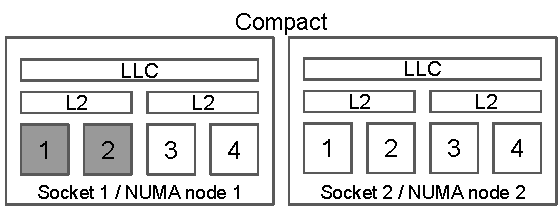
\includegraphics[width=0.48\textwidth,trim=0 0 0 17,clip]{figures/sharingAwareThreadMapping/Compact.pdf}
	}%
	\subfigure[Scatter.]{
		\label{fig:MappingStrategyScatter}
		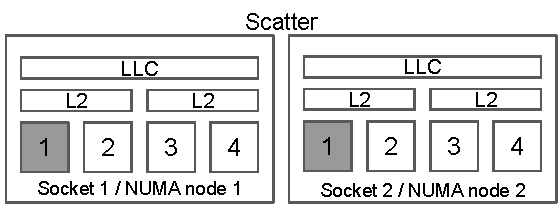
\includegraphics[width=0.48\textwidth,trim=0 0 0 17,clip]{figures/sharingAwareThreadMapping/Scatter.pdf}
	}%
\\
	\subfigure[Round-Robin.]{
		\label{fig:MappingStrategyRR}
		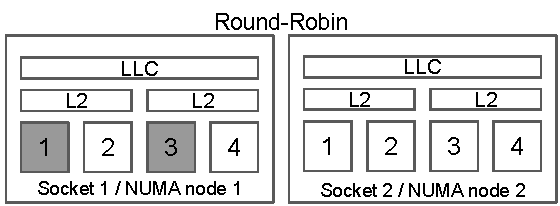
\includegraphics[width=0.48\textwidth,trim=0 0 0 17,clip]{figures/sharingAwareThreadMapping/RoundRobin.pdf}
	}%
	\caption{Thread mapping strategies.}
	\label{fig:MappingStrategy}
\end{figure}

Each application was executed 10~times using different mapping strategies:
\begin{itemize}
	\item \textbf{Linux} is the default Linux CFS scheduler~\cite{Wong:2008} used as our baseline.
	\item \textbf{Compact} places threads on sibling cores that share all cache levels, thus potentially reducing the data access latency if neighboring threads communicate~\cite{Castro:2014} (\figurename~\ref{fig:MappingStrategyCompact}).
	\item \textbf{Scatter} distributes threads across different processors, avoiding cache sharing, thus, reducing memory contention~\cite{Castro:2014} (\figurename~\ref{fig:MappingStrategyScatter}).
	\item \textbf{Round-Robin} is a mix between compact and scatter, where only the last level of cache is shared~\cite{Castro:2014} (\figurename~\ref{fig:MappingStrategyRR}).
	\item \textbf{Static-SharingAware~(SSA)} is our proposed static  approach. We first trace the behavior of each application in order to determine the communication pattern. Then, we calculate the new thread mapping offline using \texttt{TopoMatch} and re-execute the application with this \textit{static} mapping, binding threads to cores using the function \mbox{\texttt{pthread\_setaffinity\_np}}. This approach has no runtime overhead, but is not able to handle changes in the application behavior (during execution or if the behavior is different between executions).
\end{itemize}

\subsection{Results on the Xeon Machine}\label{sect:staticThreadMapXeon}

\figurename~\ref{fig:ResultsStaticXeon} shows the execution time (in seconds) on the Xeon machine. Also, each bar shows the average and a confidence interval of 95\%. The Static-SharingAware approach will be abbreviated as SSA in the discussion. Percentages of improvement are always compared to Linux, if not specified.

\begin{figure}[!bt]
	\centering
	\subfigure{
		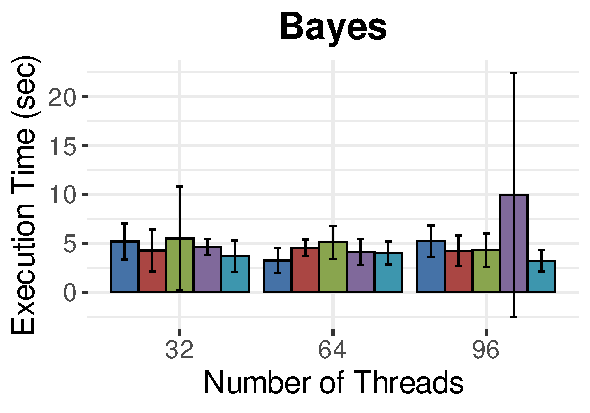
\includegraphics[width=\oneTPage\textwidth]{figures/sharingAwareThreadMapping/static/xeon/Bayes_time.pdf}
	}
	\subfigure{
		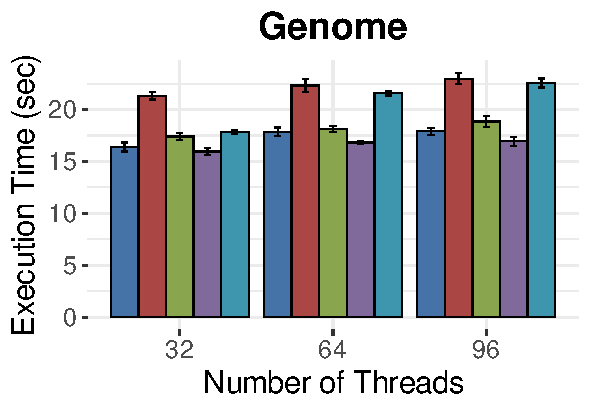
\includegraphics[width=\oneTPage\textwidth]{figures/sharingAwareThreadMapping/static/xeon/Genome_time.pdf}
	}
	\subfigure{
		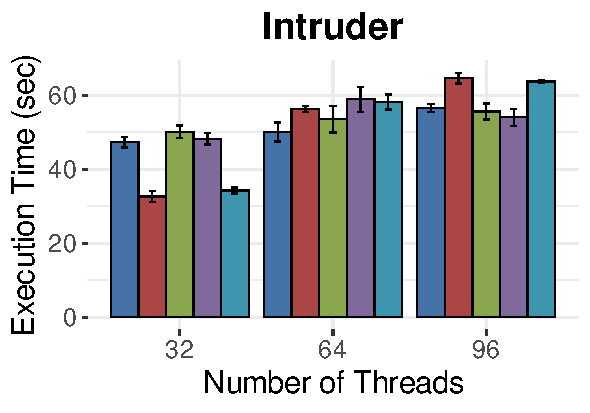
\includegraphics[width=\oneTPage\textwidth]{figures/sharingAwareThreadMapping/static/xeon/Intruder_time.pdf}
	}
	\\
	\subfigure{
		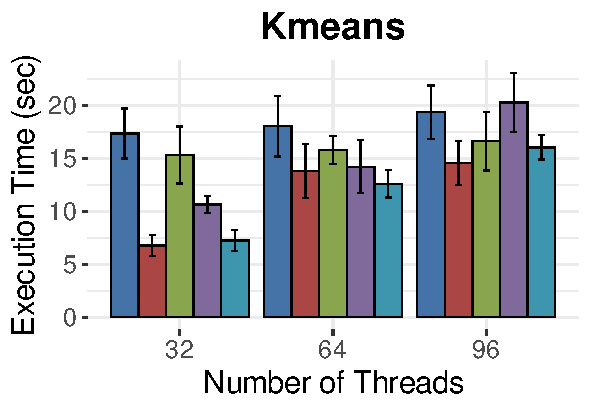
\includegraphics[width=\oneTPage\textwidth]{figures/sharingAwareThreadMapping/static/xeon/Kmeans_time.pdf}
	}
	\subfigure{
		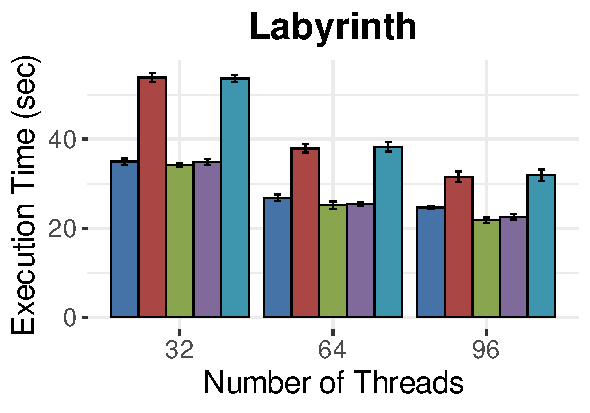
\includegraphics[width=\oneTPage\textwidth]{figures/sharingAwareThreadMapping/static/xeon/Labyrinth_time.pdf}
	}
	\subfigure{
		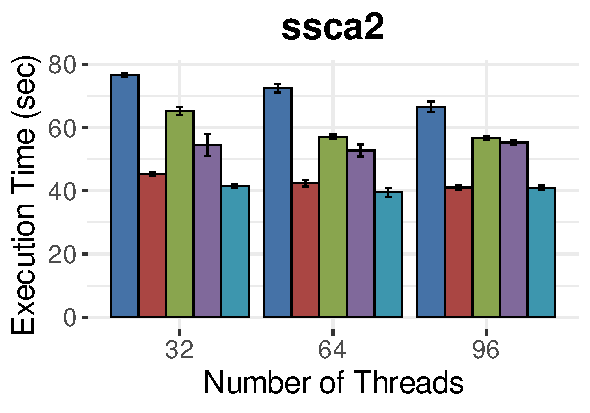
\includegraphics[width=\oneTPage\textwidth]{figures/sharingAwareThreadMapping/static/xeon/ssca2_time.pdf}
	}
	\\
	\subfigure{
		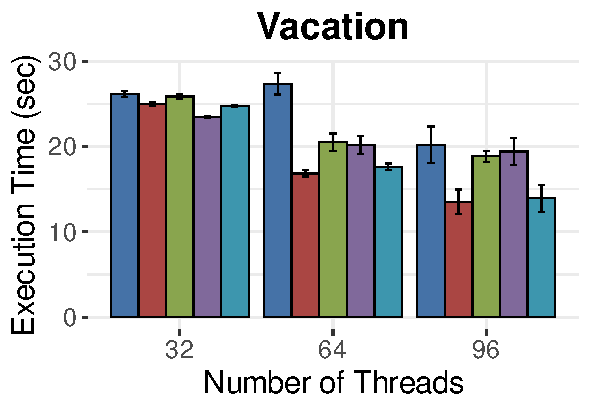
\includegraphics[width=\oneTPage\textwidth]{figures/sharingAwareThreadMapping/static/xeon/Vacation_time.pdf}
	}
	\subfigure{
		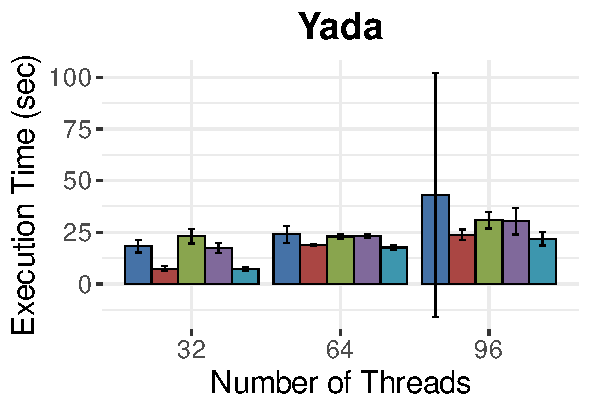
\includegraphics[width=\oneTPage\textwidth]{figures/sharingAwareThreadMapping/static/xeon/Yada_time.pdf}
	}
	\subfigure{
		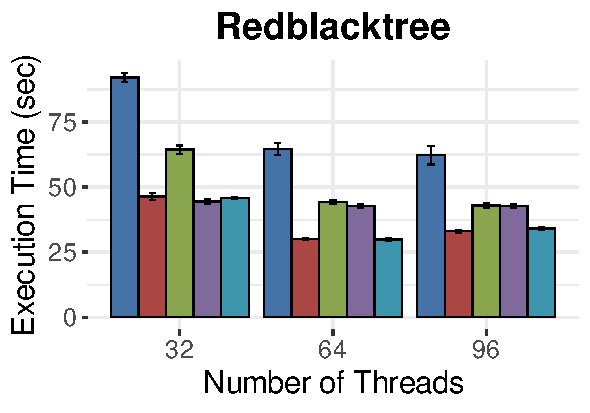
\includegraphics[width=\oneTPage\textwidth]{figures/sharingAwareThreadMapping/static/xeon/Redblacktree_time.pdf}
	}
	\\
	\subfigure{
		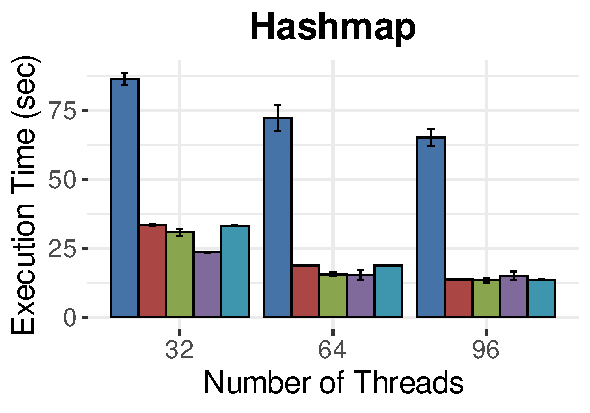
\includegraphics[width=\oneTPage\textwidth]{figures/sharingAwareThreadMapping/static/xeon/Hashmap_time.pdf}
	}
	\subfigure {
		% \includegraphics[width=\oneTPage\textwidth]{graphs/legend_h.pdf}}
		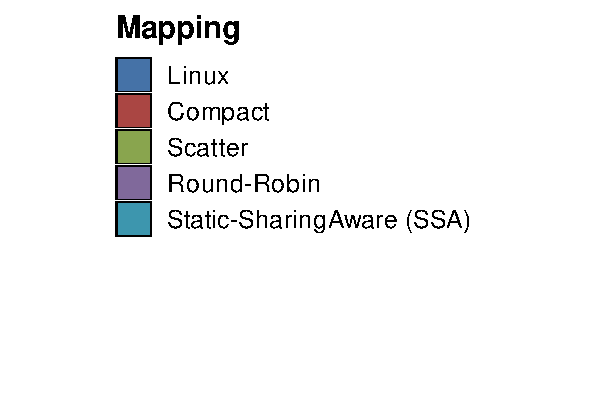
\includegraphics[width=\oneTPage\textwidth]{figures/sharingAwareThreadMapping/static/legend.pdf}}
	\caption{Execution time results on the Xeon machine.}
	\label{fig:ResultsStaticXeon}
\end{figure}

\emph{Bayes} does not present a deterministic behavior, and it is not suitable to compare execution times as the order of commits at the beginning of an execution affects the final execution time~\cite{Ruan:2014}. Thus, we will not discuss the results of this application.

\emph{Genome} has low contention and spends lots of time inside transactions \cite{STAMP}. This application is not suitable for sharing-aware thread mapping. Even though threads with higher IDs have a well-defined pattern (Section~\ref{sect:StampMatrices}), it was not enough to put them closer to increase the performance. In fact, SSA decreased the performance when compared to Linux. Round-robin had better performance gains in all scenarios. As observed by \citeNamesYearPar{Castro:2014}, transactions in \emph{genome} access disjoint data most of time, hence the low contention. Thus, it is better to map threads in order to keep more cache available for each thread, i.e., a Scatter or Round-Robin mapping or similar.

\emph{Intruder} has high contention and spends medium time inside transactions~\cite{STAMP}. SSA was the best mapping in 32 threads, achieving performance gains of 27.54\%. However, for other thread numbers, and mainly for 96 treads, SSA decreased the performance. 

\emph{Kmeans} has low contention and spends little time inside transactions \cite{STAMP}. For this application, SSA achieved good results in all thread configurations. The best performance gain of 58.28\% appeared on 32 threads. For 96 threads the performance improvement of SSA was 17.14\%, with Compact performing better (24.73\%).

\emph{Labyrinth} has high contention and spends lots of time inside transactions~\cite{STAMP}. Although this application has very different contention from \emph{genome}, the results were similar. In that case, SSA and Compact decreased the performance, with Scatter and Round-robin having similar results. It is worth noting that the best mapping configurations performed similarly to Linux.

\emph{Ssca2} has low contention, spending little time inside transactions \cite{STAMP}. Similar to \emph{kmeans}, for this application SSA delivered the highest performance gain for all thread numbers used. We have a similar performance gain of 65\% for 32 and 64 threads, and 38.5\% for 96 threads.

\emph{Vacation} has medium contention and spends high time inside transactions~\cite{STAMP}. For 32 threads, all mappings have similar results, with scatter performing slightly better. However, for 64 and 96 threads SSA had the highest performance gain of 35.55\% and 31\% respectively.

\emph{Yada} has medium contention and spends a lot of time inside transactions \cite{STAMP}. This is another example of an application where SSA had a good performance in all thread configurations. The highest performance gain was achieved under 32 threads, with 61.20\%. %Nevertheless, using 96 threads we had an expressive \new{performance improvement} of 49\% with SSA.

The last two micro-benchmarks, \emph{Hashmap} and \emph{Redblacktree} have a very similar communication pattern (Section~\ref{sect:StampMatrices}), where communication occurs often between neighboring threads. In \emph{Redblacktree}, SSA had the highest performance gain in 64 and 96 threads (53.9\% and 45.34\% respectively). In \emph{Hashmap}, Linux had a poor performance, with all thread configurations delivering expressive performance improvements. Under 96 threads, SSA had performance gains of 79.2\%.


\subsection{Results on the Opteron Machine}

\figurename~\ref{fig:ResultsStaticOpteron} shows the performance results on Opteron. Since the characteristics of the benchmarks were already discussed in the previous section, we will only discuss the performance results.

\begin{figure}[!tb]
	\centering
	\subfigure{
		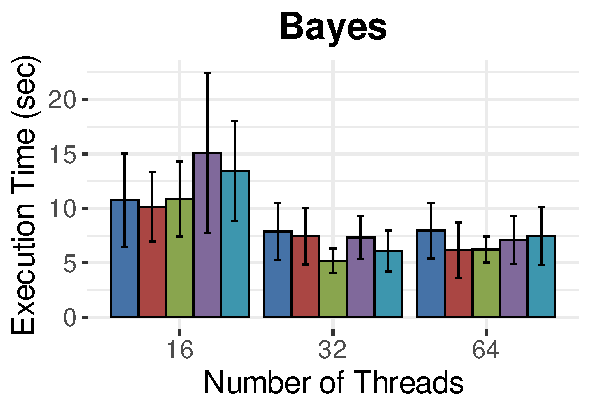
\includegraphics[width=\oneTPage\textwidth]{figures/sharingAwareThreadMapping/static/opteron/Bayes_time.pdf}
	}
	\subfigure{
		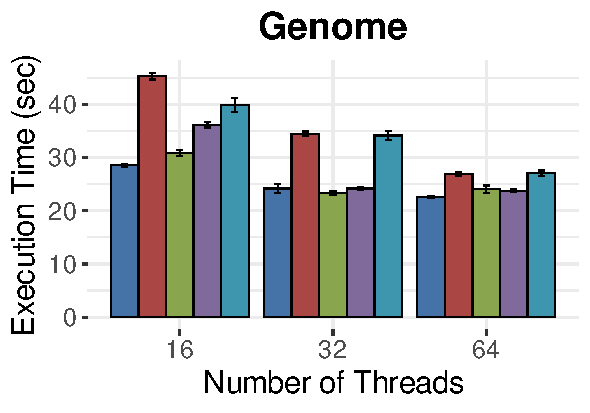
\includegraphics[width=\oneTPage\textwidth]{figures/sharingAwareThreadMapping/static/opteron/Genome_time.pdf}
	}
	\subfigure{
		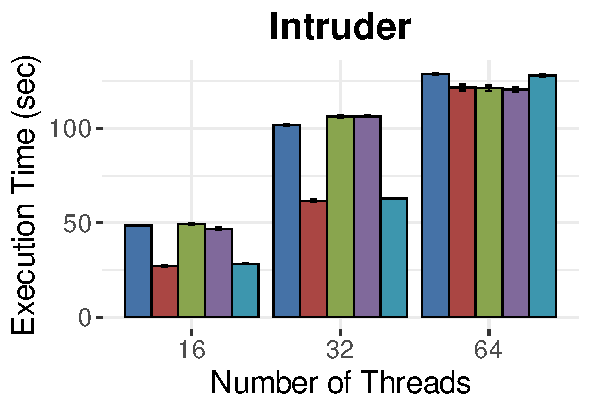
\includegraphics[width=\oneTPage\textwidth]{figures/sharingAwareThreadMapping/static/opteron/Intruder_time.pdf}
	}
	\\
	\subfigure{
		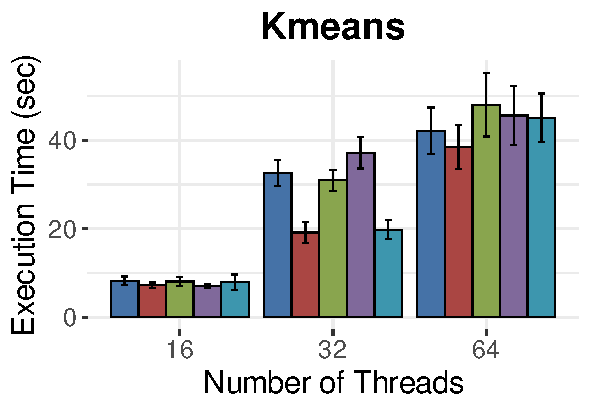
\includegraphics[width=\oneTPage\textwidth]{figures/sharingAwareThreadMapping/static/opteron/Kmeans_time.pdf}
	}
	\subfigure{
		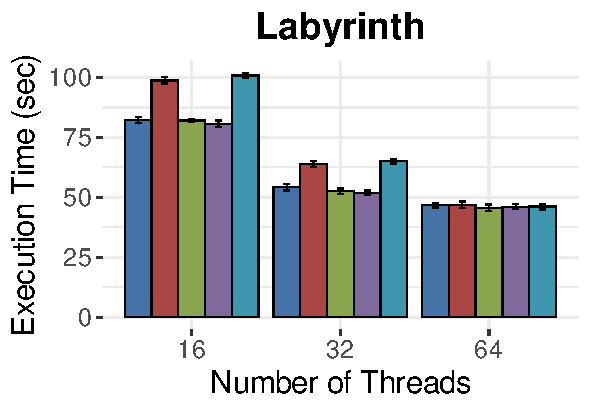
\includegraphics[width=\oneTPage\textwidth]{figures/sharingAwareThreadMapping/static/opteron/Labyrinth_time.pdf}
	}
	\subfigure{
		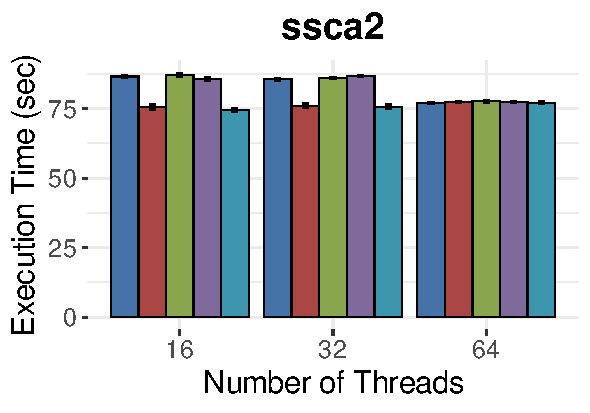
\includegraphics[width=\oneTPage\textwidth]{figures/sharingAwareThreadMapping/static/opteron/ssca2_time.pdf}
	}
	\\
	\subfigure{
		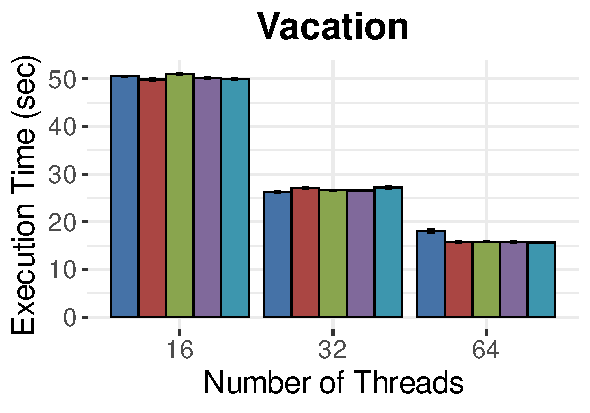
\includegraphics[width=\oneTPage\textwidth]{figures/sharingAwareThreadMapping/static/opteron/Vacation_time.pdf}
	}
	\subfigure{
		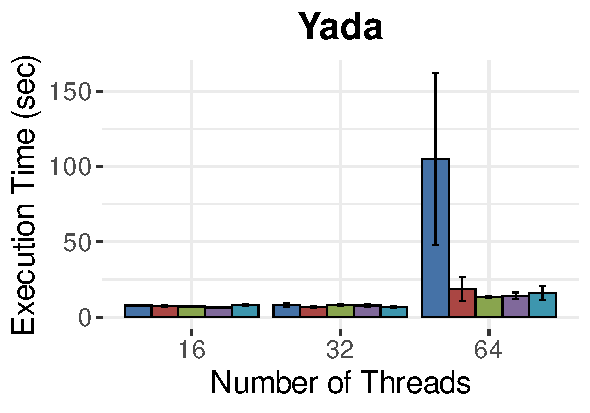
\includegraphics[width=\oneTPage\textwidth]{figures/sharingAwareThreadMapping/static/opteron/Yada_time.pdf}
	}
	\subfigure{
		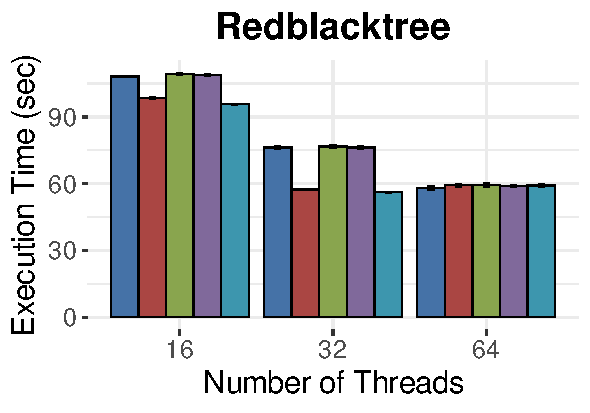
\includegraphics[width=\oneTPage\textwidth]{figures/sharingAwareThreadMapping/static/opteron/Redblacktree_time.pdf}
	}
	\\
	\subfigure{
		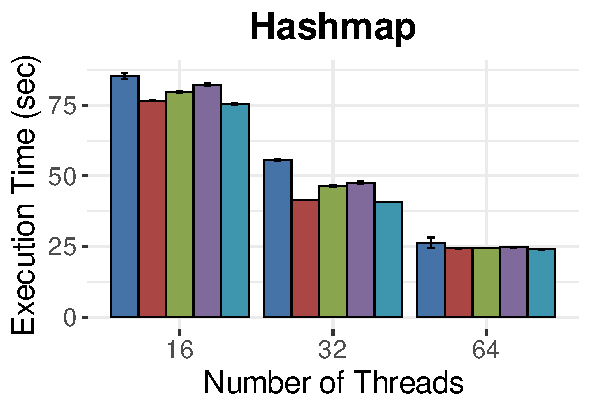
\includegraphics[width=\oneTPage\textwidth]{figures/sharingAwareThreadMapping/static/opteron/Hashmap_time.pdf}
	}
	\subfigure {
		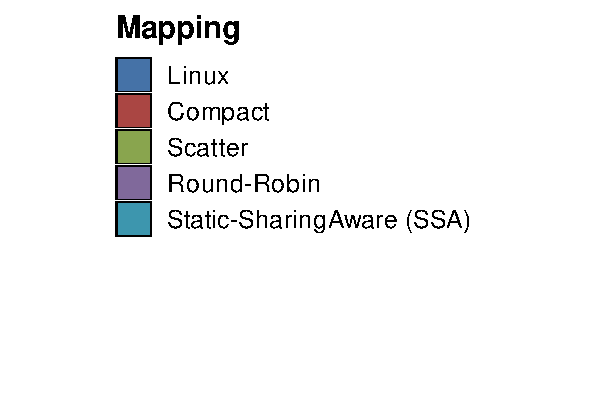
\includegraphics[width=\oneTPage\textwidth]{figures/sharingAwareThreadMapping/static/legend.pdf}}
	\caption{Execution time results on the Opteron Machine.}
	\label{fig:ResultsStaticOpteron}
\end{figure}

For \emph{Genome}, it is possible to observe the same behavior on the Xeon machine, where SSA decreases the performance. However, for this machine Scatter was not the best mapping in all thread numbers. For 16 threads Linux performed better, and slightly similar to Scatter and Round-Robin on 32 and 64 threads.

In the Xeon machine, \emph{Intruder} has good performance only with 32 threads. Similarly, in Opteron, the performance gain of SSA was expressive with 32 threads (38.26\%). With 16 threads, the performance improvement of SSA was even better, 41.57\%.  However, with 64 threads the performance started to decrease with SSA. Hence, this application is suitable for a sharing-aware thread mapping only with low thread numbers.

In \emph{Kmeans}, SSA had an expressive performance improvement of 39.25\% under 32 threads. For 16 threads, all mapping performed similarly. Under 64 threads, Compact was the best mapping.

In \emph{Labyrinth}, it is possible to observe the same results as in the Xeon machine. This is another application that is not suitable for sharing-aware thread mapping. SSA and Compact decreased performance with 16 and 32 threads. Under 64 threads all mappings performed similarly.

For \emph{Ssca2}, SSA delivered the highest performance gain for all thread numbers used, mainly for 16 (13.8\%) and 32 threads (11.52\%). Hence, the results were similar to the Xeon machine.

\emph{Vacation} had a very different behavior compared to the Xeon machine. In Opteron, no mapping had a great impact on the final performance. All performed slightly similar.

\emph{Yada} is similar to \emph{Vacation}. However, in 64 threads, the Linux performance was poor, increasing execution time in more than 10$\times$.

Overall, the last two micro-benchmarks, \emph{Hashmap} and \emph{Redblacktree} have a
very similar performance to the Xeon machine. SSA was the best mapping in both 16 and 32 threads. In \emph{Redblacktree} the performance gains were 11.47\% and 26.31\% respectively, whereas in \emph{Hashmap} it was 11.62\% and 26.54\%.

\subsection{Discussion}

%On the Opteron machine, the best speedup over Linux was achieved by \emph{Yada} using 64 threads (85.8\%) and by Intruder using 16 threads (39.4\%). On the Xeon machine, the highest speedup was achieved by \emph{Hashmap}, achieving gains of 77.7\% over Linux.

As shown in the results, not all applications are suitable for sharing-aware thread mapping. On both machines, \emph{Genome} and \emph{Labyrinth} prefer a mapping that reduces memory contention, such as Scatter. However, overall, SSA improved the performance of many applications, being the mapping with the highest performance improvement. In the Xeon machine the highest performance gains of SSA over Linux were achieved by \emph{Hashmap} using 96 threads (79.2\%) and by \emph{Yada} using 32 threads (61.2\%). On the Opteron machine, the highest performance gains were achieved by \emph{Yada} using 32 threads, achieving gains of 84.82\% over Linux and by Intruder (41.57\%).

%In Opteron machine, with exception of a few application, using all threads, including the SMT ones, all mappings performed similar. This can be explained because using all threads we have other challenges, such as ....

It is worth noting that only transactional operations were tracked to determine the sharing behavior. The intuition is that if a memory location is shared by more than one thread, it will be protected by transactional operations.

To summarize, \tablename~\ref{tab:resultsStatic} shows the average performance gains of each mechanism over Linux, taking into consideration all applications and thread configurations.
\begin{table}[!tb]
	\centering
	\caption{Average performance gains of each mechanism over Linux.}
	\label{tab:resultsStatic}
	\begin{tabular}{lrrrrr}
		\toprule
		\textbf{Machine}  & \textbf{Compact} & \textbf{Scatter} & \textbf{Round\textbf{}Robin} & \textbf{SSA}  \\
		\midrule
		\textbf{Xeon}   & 15.88\%          & 13.14\%          & 14.50\%            & 22.32\%   \\
		\textbf{Opteron} & 7.96\%           & 5.86\%           & 3.15\%            & 6.50\%      \\
		\bottomrule
	\end{tabular}
\end{table}
As shown in Section~\ref{sec:improvements} in the experiment of the array sum, the Xeon machine is more sensitive to a sharing-aware thread mapping, since \texttt{TopoMatch} prioritizes the placement of threads first inside the same socket. As explained, this machine has a larger LLC cache on each socket, showing higher gains than Opteron.

It is worth noting that the experiments so far only showed that some applications are suitable for sharing-aware thread mapping and others are not. However, at this point, we do not know which kind of characteristics make an application suitable for a sharing-aware thread mapping. In the next Section~(\ref{sect:onlineThreadMapping}), we intend to do thread mapping during runtime. Hence, additional experiments will be made in order to discover the characteristics that make an application suitable for a sharing-aware thread mapping.

\section{Online thread mapping}\label{sect:onlineThreadMapping}

Although the experiments of the previous section~(\ref{sect:staticThreadMap}) show that a static sharing-aware thread mapping is sufficient to improve the performance of STM applications, this section presents an online mechanism, called \emph{STMap}. Contrary to SSA, STMap does not need prior information about the sharing behavior of the application, since the detection of sharing behavior and thread migration are performed based on information gathered solely during execution.

\subsection{Reducing the overhead of online detection}\label{sec:lessoverhead}

Since we are interested in detecting communication and performing thread mapping online, keeping track of every accessed address would be infeasible, due to the high overhead added to the application. Hence we use the concept of \emph{sampling}. The goal is to choose a \emph{sampling interval} (SI) with a high accuracy but low overhead. To choose the SI, we ran an experiment using all eight benchmarks from  \texttt{STAMP}. %\texttt{STAMP} is a collection of realistic workloads, covering a wide range of transactional execution cases.

We start with a sampling interval of zero, i.e., all addresses are sampled in the communication matrix. The next sampling interval is 10, i.e., only execute Algorithm~\ref{alg:detectcomm}~(Chapter~\ref{chap:mechanism}) once for every ten addresses accessed. The other sampling intervals are always ten times the previous one. To avoid contention, every thread has their own sampling interval counter.

%Also, this approach allows having a more accurate mechanism. If the SI were global, in a worst-case, the Algorithm~\ref{alg:detectcomm} would be triggered always by the same thread, and it would not be possible do detect a communication pattern.

%/home/douglas/GitRepo/PhDRepo/02.OnlineThreadMapping/stamp-m-32TXeon
\begin{figure}[!t]
	\centering
	\subfigure[Overhead.]{
		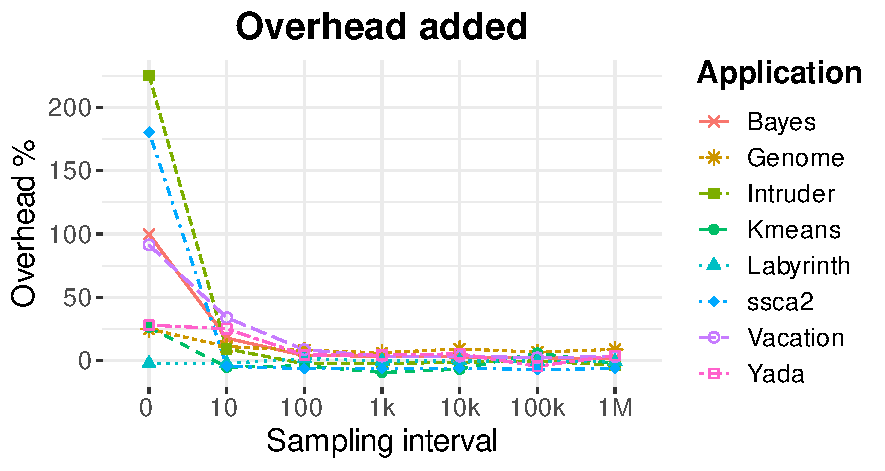
\includegraphics[width=0.9\textwidth]{figures/sharingAwareThreadMapping/online/overhead/Overhead.pdf}
		\label{fig:sampleIntervals}
	}
\\
	\subfigure[MSE.]{
		\label{fig:MSEOverSample}
		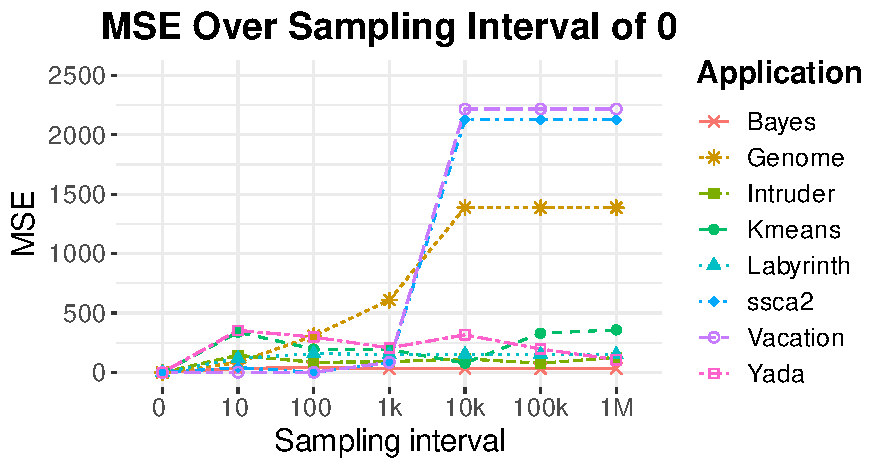
\includegraphics[width=0.9\textwidth]{figures/sharingAwareThreadMapping/online/overhead/MSE.pdf}
	}
	\\
%	\centering
%	\subfigure {
%		
\includegraphics[width=0.9\textwidth]{figures/sharingAwareThreadMapping/online/overhead/legend.pdf}
%	}
	\caption{Overhead and MSE when varying the sampling interval.
	}
	\label{fig:arraySumGraphs}
\end{figure}

\figurename~\ref{fig:sampleIntervals} shows the overhead results. Applications with many addresses accessed such as \emph{Intruder} and \emph{ssca2}
have a high overhead even when using a sampling interval of 10. We also studied how the accuracy of the collected communication matrices is affected by each SI. We used the mean squared error (MSE)~(Section \ref{sec:MSE}) as a metric to compare the resulting matrices of each sampling interval, comparing them to the sampling interval of 0.

\figurename~\ref{fig:MSEOverSample} shows the results. Lower values are better. Analyzing the graphs, we chose a sampling interval of \textbf{100}, where the applications presented the best trade-off between overhead and accuracy.

Finally, we need to choose the \emph{mapping interval}~(MI), i.e., when the new thread mapping should be calculated. Migrating threads incurs an overhead due to cache misses and other collateral effects. In NUMA machines, these effects can be even worse, due to messages of cache invalidation between nodes. Hence, our idea is to reduce the number of times that thread mapping is performed. We need to choose a mapping interval as early as possible, taking into consideration the trade-off between accuracy and overhead. Our mapping interval is based on the total number of accessed addresses (not just the number of sampled addresses). Thus, we made a previous analysis of the applications and chose an MI of \textbf{100,000} (more details about these thresholds will be explained in Section \ref{sec:calculatemap}). Hence, we calculate the new thread mapping when the application accessed `'mapping interval'' addresses. Again, to avoid contention we decided to track the total of accessed addresses of only one thread.

\subsection{Calculating the mapping}\label{sec:calculatemap}

To calculate the thread mapping, the communication matrix created by the Algorithm~\ref{alg:detectcomm} is used as input for the \texttt{TopoMatch} mapping algorithm~\cite{TopoMatch}. Using the generated mapping, threads are pinned to cores using the \mbox{\texttt{pthread\_setaffinity\_np}} function. \texttt{TopoMatch} has an important feature
for NUMA machines: when calculating the new thread mapping, it tries to minimize the communication costs between sockets/nodes. Hence, it prioritizes the placement of threads first inside the same socket.

As showed in the experiments with SSA~(Section~\ref{sect:staticThreadMap}), not all STM applications are suitable for sharing-aware thread mapping. Thus, we use a heuristic which is measured before calculating a new thread mapping to verify if the application would benefit from using the proposed approach. To define a heuristic, we analyzed different application characteristics. The idea is to try to discover common characteristics between applications where the sharing-aware thread mapping decreased the performance. Similar to the experiments made in Chapter~\ref{chap:charact}, we use \texttt{STAMP} applications for this analysis, since it was developed to represent realistic workload characteristics and it covers a wide range of transactional behavior. To have a low overhead mechanism, we tried as much as possible to measure the desired characteristics on the main thread, avoiding thread synchronization. The initial analyzed characteristics were: the total numbers of commits and aborts, the total number of transactions, the average size of the read and write-set and the commit and abort ratios. Also, we analyzed two global metrics: the total number of accessed addresses and the amount of distinct addresses accessed. Based on Section~\ref{sect:staticThreadMap} we already know the kinds of applications that are not suitable for sharing-aware thread mapping. Hence, we are interested in finding a heuristic to disable the mechanism on such applications. Analyzing the collected characteristics, we decided to take into consideration the number of distinct addresses (\textit{da}) accessed by all threads and the commit and abort ratio (\textit{cr} and \textit{ar}) of thread 1. Besides, we used the same experiment to decide the mapping interval, i.e., the metric used to decide when a new thread mapping should be calculated.
\begin{table}[!tb]
	\centering
	\caption{Characteristics used to define the heuristic and the mapping interval.}
	\label{tab:characApplications}
	\small
	\begin{tabular}{@{}lrrrrrrrrr@{}}
		\toprule
		& \multicolumn{3}{r}{MI: 10K, 32 Threads} & \multicolumn{3}{r}{MI: 50K, 32 Threads} & \multicolumn{3}{r}{MI: 50K, 96 Threads} \\
		\cmidrule(lr){2-4} \cmidrule(lr){5-7} \cmidrule(l){8-10}
		Application & \textit{da}          & \textit{cr}         & \textit{ar}        & \textit{da}           & \textit{cr}        & \textit{ar}        & \textit{da}           & \textit{cr}        & \textit{ar}        \\ \midrule
		bayes        & ---           & ---          & ---         & ---            & ---         & ---         & ---            & ---         & ---         \\
		genome       & 476         & 0.35       & 0.65      & 20,698       & 0.96     & 0.04         & 6,816        & 0.00         & 0.00         \\
		intruder     & 593         & 0.00       & 0.00     & 1,922        & 0.00      & 0.00         & 1,314        & 0.00         & 0.00         \\
		kmeans       & 19          & 0.06       & 0.94     & 21           & 0.04      & 0.96      & 20           & 0.00         & 0.00         \\
		labyrinth    & 4,279       & 1.00       & 0.00     & 14,144       & 0.70      & 0.30      & ---            & ---         & ---         \\
		ssca2        & 2,833       & 1.00       & 0.00     & 21,363       & 1.00      & 0.00         & 69,087       & 1.00         & 0.00         \\
		vacation     & 2,447       & 0.00       & 0.00     & 10,622       & 0.00      & 0.00         & 4,911        & 0.00         & 0.00         \\
		yada         & 989         & 0.00       & 0.00     & 1,857        & 0.01      & 0.99      & 7,075        & 0.00         & 0.00         \\
		redblacktree & 604         & 0.00       & 0.00     & 2,832        & 0.00      & 0.00         & 10,232       & 0.74      & 0.26      \\
		hashmap      & 216         & 0.00       & 0.00     & 1,692        & 0.00      & 0.00         & 35,290       & 1.00         & 0.00         \\ \bottomrule
	\end{tabular}
\end{table}
\tablename~\ref{tab:characApplications} shows the chosen metrics using different thread numbers and MI's. It is worth noting that in \emph{bayes} it was not possible to collect the information, even when using a mapping interval of 10,000 addresses. This application accesses a very low number of addresses. Nevertheless, this application is not adequate to compare execution time, since its behavior is not deterministic~\cite{Ruan:2014}. When both \textit{cr} and \textit{ar} are zero in \tablename~\ref{tab:characApplications}, it means that the application does not completed any transactions when the MI was reached. In that case, it was not possible to calculate the ratios. When using a mapping interval of 50,000 it was possible to define a heuristic to disable the thread mapping for the applications that were not suitable for sharing-aware thread mapping. In the case of  \texttt{STAMP}, the applications less suitable for sharing-aware thread mapping are \emph{Genome}, \emph{Intruder} and \emph{Labyrinth}. Since the applications that are not sensitive to our mechanism present a similar behavior on the analyzed characteristics, we expect that other applications that are not suitable for a sharing-aware thread mapping present the same characteristics. Hence, the heuristic is shown in Algorithm~\ref{alg:enableMappig}.

\begin{algorithm}[!tb]
	\caption{Heuristic used to determine if the thread mapping should be calculated}\label{alg:enableMappig}
	\small
	\begin{algorithmic}[1]
		\Function{enableMapping}{}
		\State $da \gets \text{getTotalDa()}$ \label{alg:emCountDa}
		\If{($da <= da\_threshold$)}
		\State \Return true   \Comment{Compute the new thread mapping }
		\Else
		\State $commits \gets \text{getTotalCommitsThread()}$ \label{alg:emCommits} \Comment{Only for thread 1}
		\State $aborts \gets \text{getTotalAbortsThread()}$ \Comment{Only for thread 1}
		\State $transactions \gets commits + aborts$
		\If{($transactions > 0$)}
		\State $cr \gets commits / transactions$
		\State $ar \gets aborts / transactions$
		\State \Return $ar > cr$ \label{alg:emARGeCR}
		\Else
		\State \Return false  \label{alg:emReturnFalse} 				\Comment{Zero transactions so far. It is not possible do calculate the ratios}
		\EndIf
		\EndIf
		\EndFunction
	\end{algorithmic}
\end{algorithm}

%The heuristic is based on the \emph{distinct address} (\texttt{da}) accessed by the application, the \emph{abort ratio} (\texttt{ar}) and \emph{commit ratio} (\texttt{cr}). Following the same intuition from MI, the \texttt{ar} and \texttt{cr} are determined only by thread 1.
%The \texttt{da} metric is global, i.e., not only based on thread 1, because we need to calculate it just one time (from the hash table, Sect. \ref{sec:detectComm}), inside the heuristic (line~\ref{alg:emCountDa}).
The \texttt{da} is calculated from the hash table (Chapter~\ref{chap:mechanism}, \figurename~\ref{fig:mechanism}), inside the heuristic (line~\ref{alg:emCountDa}). The value of da\_threshold was set to \textbf{10,000} based on the analysis of the data in \tablename~\ref{tab:characApplications}. Thus, if the application had accessed less than 10,000 distinct addresses, the new thread mapping should be calculated. The intuition used here is that if there many distinct addresses accessed, the application probably does not have a well-defined communication pattern between threads. However, if there are more than 10,000 distinct addresses, the commit and abort ratio of thread 1 are used for determining if the mechanism should be disabled (lines \ref{alg:emCommits} to \ref{alg:emReturnFalse}). The intuition here is based on the works of \citeNamesYearPar{Castro:2014} and \citeNamesYearPar{Chan:2015}, who determined that if the abort ratio is high, then the application is accessing too much shared data. Thus, putting them closer would increase cache sharing between the shared data, which is one of the main objectives of sharing-aware thread mapping. For these reasons, if the  \texttt{ar} is higher than the  \texttt{cr}, the new thread mapping should be calculated (line~\ref{alg:emARGeCR}).

A final remark is related to the mapping interval when using 96 threads. The Xeon machine that will be used for the experiments has 96 physical cores. Analyzing the data for this configuration in \tablename~\ref{tab:characApplications}, we do not see the same \textit{da} of 10,000 for the application that we are interested in disabling the mechanism. Overall, the \textit{da} was lower. Hence, our idea is also to include in the experiments a higher mapping interval, in that case, 100,000 addresses. %On \emph{Labyrinth}, the application access less than 100,000 addresses in thread 1. Hence, the thread mapping will be not triggered for this configuration of MI and number of threads.

\subsection{Final algorithm}\label{sect:finalAlgorithmOnlineMap}

In this Section, we present the final algorithm to detect and perform the thread mapping dynamically (Algorithm~\ref{alg:commAndMap}). Also, \figurename~\ref{fig:stmap-fluxogram} shows the updated version of the basic mechanism to detect the communication pattern, proposed in Chapter~\ref{chap:mechanism}.

\begin{figure}[!ht]
	%https://docs.google.com/presentation/d/1qCPtTkkpekSZeEv-8jGUWJD9Wbn4KpB9ZLX9Z3cgqcU/edit#slide=id.g961e369ddb_3_0
	\centering
	\fbox{
		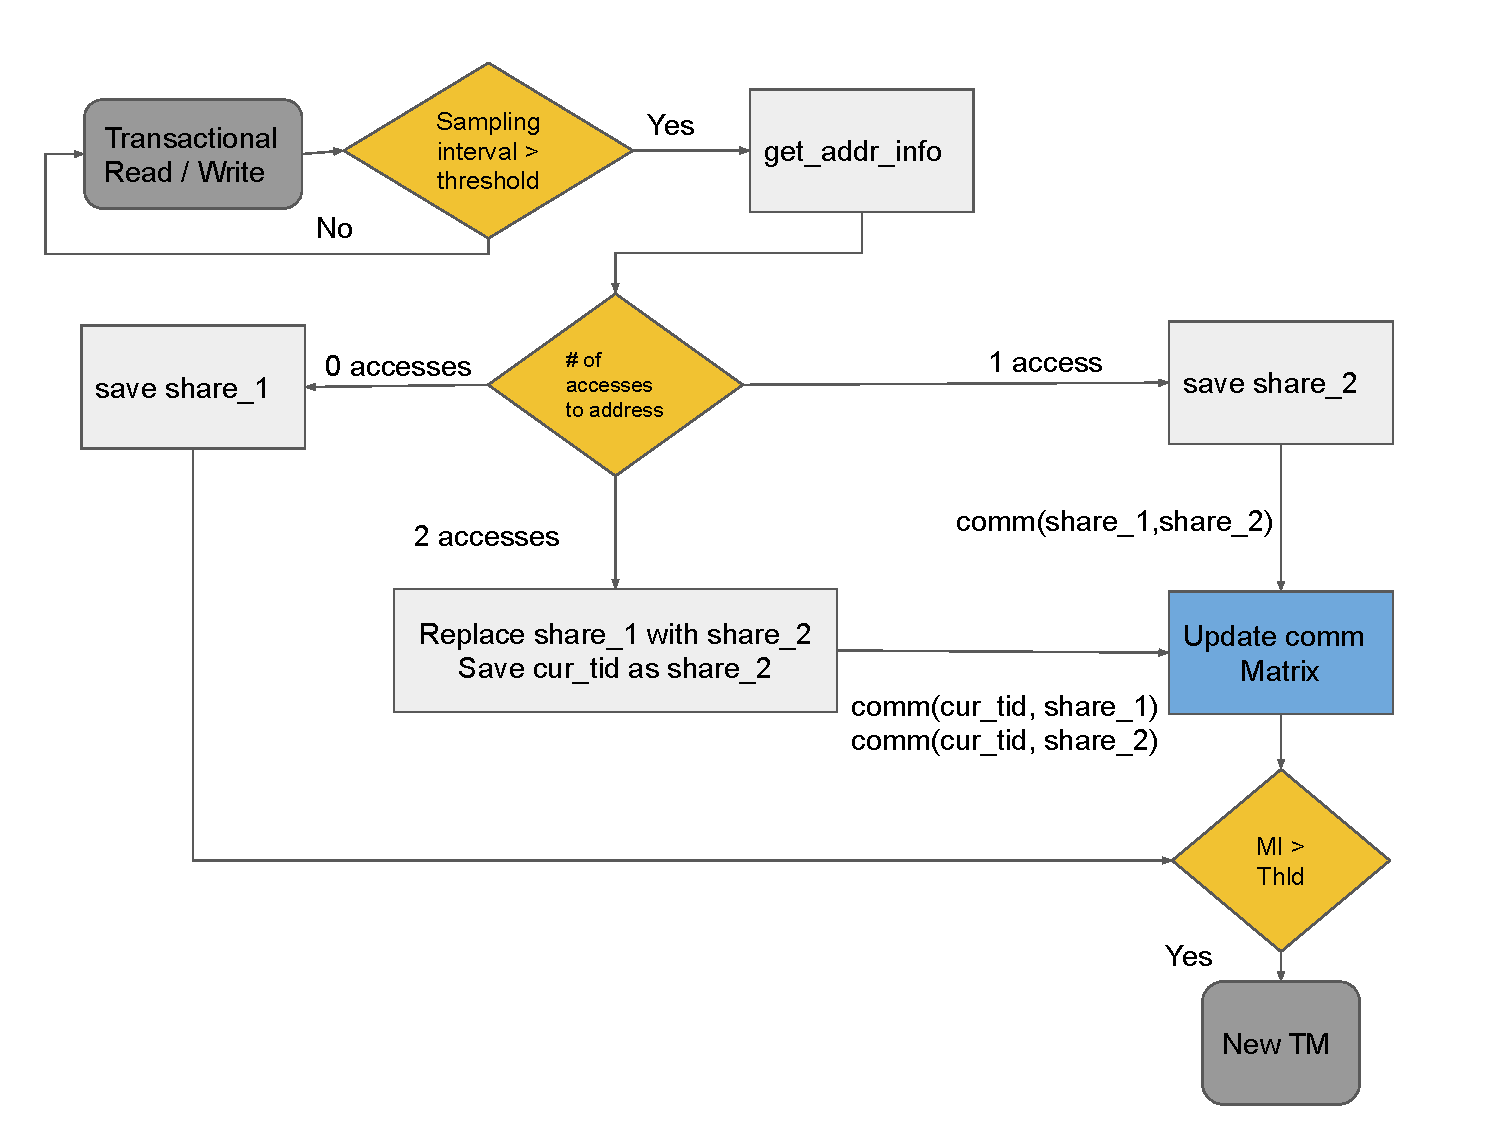
\includegraphics[width=\fullImageWidth\textwidth,trim=20 0 30 0,clip]{figures/sharingAwareThreadMapping/STMap-Fluxogram.pdf}
	}
	\caption{Flowchart of the proposed mechanism to detect and perform thread mapping during runtime. In this Figure, Thld stands for threshold and TM for thread mapping.}
	\label{fig:stmap-fluxogram}
\end{figure}

%
\begin{algorithm}[!ht]
	\caption{Triggering communication events and thread mapping.}\label{alg:commAndMap}
	\small
	\begin{algorithmic}[1]
		\Require
		\Statex \textbf{addr}: memory address being accessed
		\Statex \textbf{tid}: thread ID of the thread that is accessing the address
		\Statex \textbf{addr\_sample} : thread private variable used to determine if is time to sample the memory address
		\Statex \textbf{total\_addr} : thread private variable used to determine if is time to trigger the thread mapping
		\Statex \textbf{si}: sample interval. Default 100
		\Statex \textbf{mi}: mapping interval. Default 100,000
		\Statex
		%	\If {($collect\_comm$)} \label{alg2:shouldcollect}
		\State $addr\_sample \gets addr\_sample + 1$ \label{alg2:incsample}
		\If{($addr\_sample > si$)}  \label{alg2:samplegreater}
		\State $addr\_sample \gets 0$ \label{alg2:zerosample}
		\State Execute algorithm \ref{alg:detectcomm}
 \Comment{Proposed in Chapter~\ref{chap:mechanism}}
		\EndIf
		%	\LineComment{To avoid high overhead, for mapping purposes, only keep track of total address accessed by thread 1}
		\If {($tid = 1$)} \label{alg2:isthreadone}
		\State $total\_addr \gets total\_addr + 1$ \label{alg2:inctotaladdr}
		\EndIf
		\If {($tid = 1$)  \textbf{and} ($total\_addr \geq mi$)} \label{alg2:istimetomap}
		%			\State $collect\_comm \gets false$ \label{alg2:disablemech}
		\If{($EnableMapping()$)} \label{alg2:callequation1}\Comment{Algorithm~\ref{alg:enableMappig}}
		\State Compute new thread mapping
		\EndIf
		\EndIf
		%		\EndIf
	\end{algorithmic}
\end{algorithm}
%
%Since we intend to perform the thread mapping only once,
%We have a special variable to control if the mapping already has been performed (line \ref{alg2:shouldcollect}). If true, the mechanism is disabled.
First, the thread private variable \texttt{addr\_sample} (line~\ref{alg2:incsample}) is incremented to verify if it is time to sample the memory access. Then, on the line~\ref{alg2:samplegreater} we verify if the counter of the current thread is greater than the sampling interval (Section~\ref{sec:lessoverhead}). If true, we zero the variable to be able to detect the next trigger time (line~\ref{alg2:zerosample}), and Algorithm~\ref{alg:detectcomm} is executed.

The next part of the algorithm controls when to perform the new thread mapping. In line \ref{alg2:isthreadone}, we determine if the current thread is the one responsible to control the total of addresses accessed, i.e., thread one. If true, we increment the thread private variable \texttt{total\_addr} (line \ref{alg2:inctotaladdr}). Thus, in line~\ref{alg2:istimetomap} the algorithm determines if it is time to trigger the new thread mapping, checking if the total of accesses is greater than or equal to the mapping interval (Section~\ref{sec:lessoverhead}). If true, %we disable the mechanism (line \ref{alg2:disablemech}) and
it is necessary to verify if the application will  benefit from a new mapping. This verification is done through the Algorithm~\ref{alg:enableMappig} (line~\ref{alg2:callequation1}). Finally, if Algorithm~\ref{alg:enableMappig} returns \emph{true}, we compute the new thread mapping according to Section~\ref{sec:calculatemap}.

\subsection{Implementation}\label{sec:onlineImplement}


We extended the implementation of the proposed mechanism to detect the sharing behavior, described in Section~\ref{sec:implement}. The extension included the Algorithm~\ref{alg:commAndMap} inside the function \texttt{stm\_write} and \texttt{stm\_load}.
%

One key aspect of the implemented mechanism is that we only trigger the thread mapping once during the execution of the application. The experiments in Chapter~\ref{chap:charact} showed that the \texttt{STAMP} applications do not present dynamic sharing behavior, i.e., they have the same sharing pattern during all execution time. For this reason, after the first mapping interval is triggered, the mechanism is disabled, stopping to collect memory access information. Nevertheless, we do not expect significant performance penalties if the mechanism is enabled during all the execution time. As shown in \figurename~\ref{fig:MSEOverSample} the chosen sampling interval of 100 represents a very small overhead to the final execution time.


\subsection{Results on the Xeon Machine}

\figurename~\ref{fig:ResultsOnlineXeon} shows the execution time (in seconds) on the Xeon machine. Also, each bar shows the average and a confidence interval of 95\%. When discussing the distinct addresses accessed and commit and abort ratios, these metrics are based on when the mapping interval was triggered. Percentages of improvement are always compared to Linux. As some results can be explained by the level of contention of each application, this information will be included again, for each application analyzed, such as in the static results discussion (Section~\ref{sect:staticThreadMapXeon}).

\begin{figure}[!bt]
	\centering
	\subfigure{
		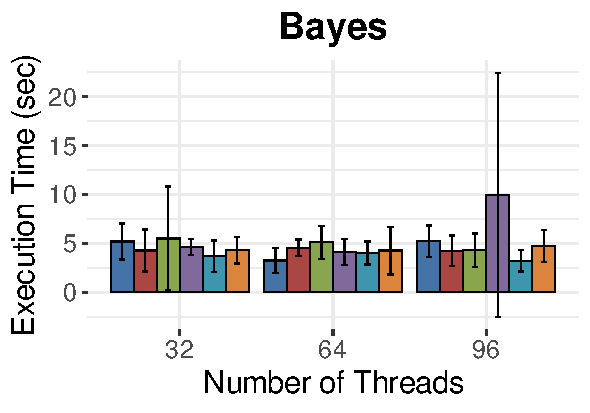
\includegraphics[width=\oneTPage\textwidth]{figures/sharingAwareThreadMapping/online/xeon/Bayes_time.pdf}
	}
	\subfigure{
		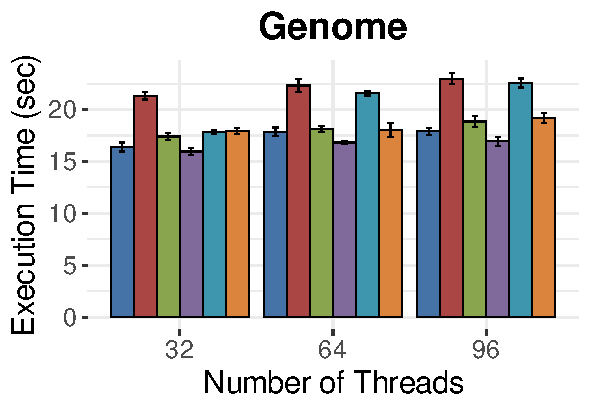
\includegraphics[width=\oneTPage\textwidth]{figures/sharingAwareThreadMapping/online/xeon/Genome_time.pdf}
	}
	\subfigure{
		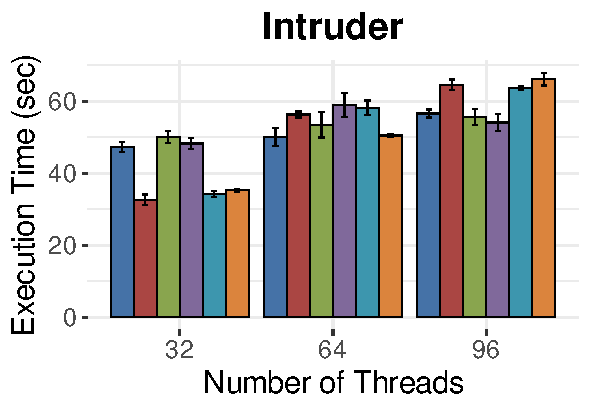
\includegraphics[width=\oneTPage\textwidth]{figures/sharingAwareThreadMapping/online/xeon/Intruder_time.pdf}
	}
	\\
	\subfigure{
		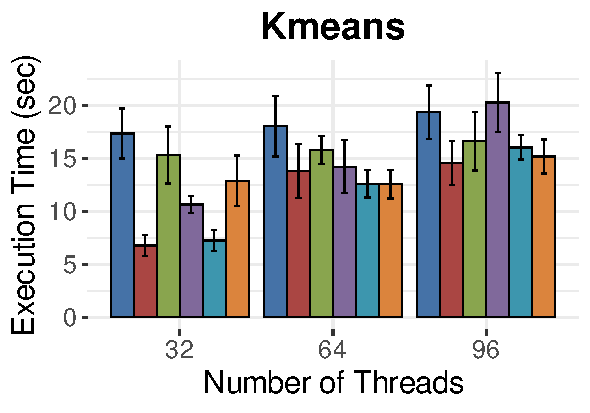
\includegraphics[width=\oneTPage\textwidth]{figures/sharingAwareThreadMapping/online/xeon/Kmeans_time.pdf}
	}
	\subfigure{
		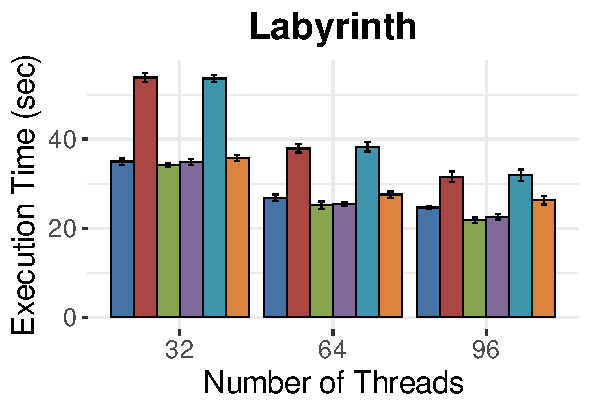
\includegraphics[width=\oneTPage\textwidth]{figures/sharingAwareThreadMapping/online/xeon/Labyrinth_time.pdf}
	}
	\subfigure{
		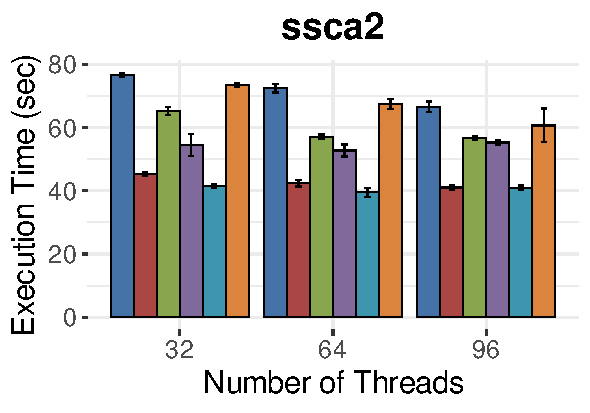
\includegraphics[width=\oneTPage\textwidth]{figures/sharingAwareThreadMapping/online/xeon/ssca2_time.pdf}
	}
	\\
	\subfigure{
		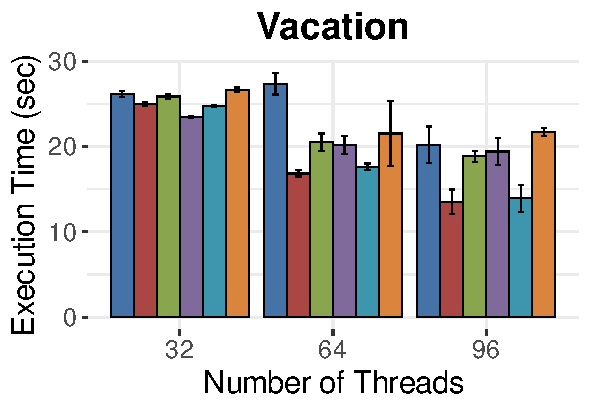
\includegraphics[width=\oneTPage\textwidth]{figures/sharingAwareThreadMapping/online/xeon/Vacation_time.pdf}
	}
	\subfigure{
		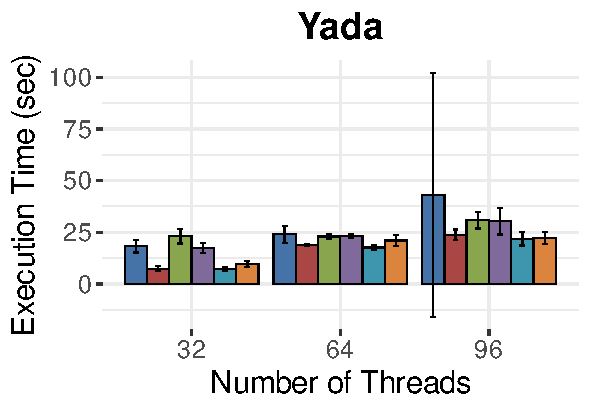
\includegraphics[width=\oneTPage\textwidth]{figures/sharingAwareThreadMapping/online/xeon/Yada_time.pdf}
	}
	\subfigure{
		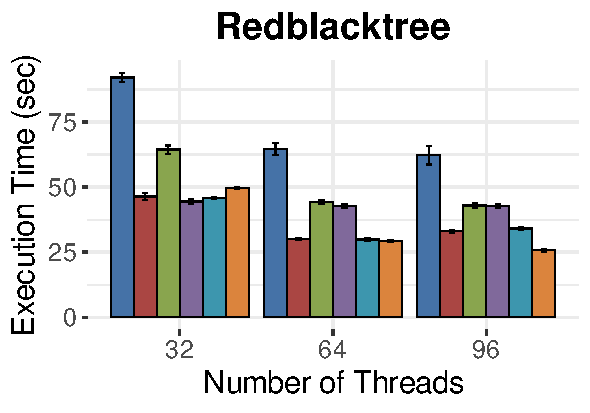
\includegraphics[width=\oneTPage\textwidth]{figures/sharingAwareThreadMapping/online/xeon/Redblacktree_time.pdf}
	}
	\\
	\subfigure{
		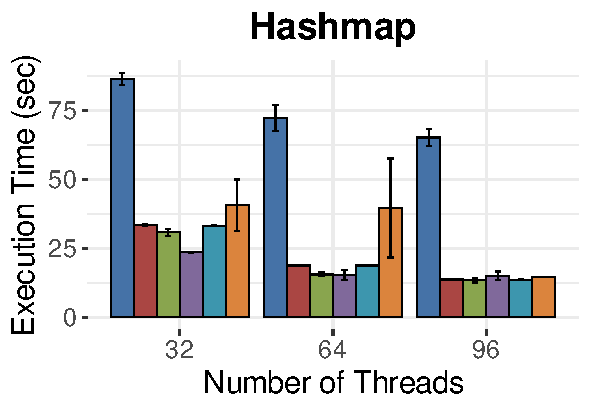
\includegraphics[width=\oneTPage\textwidth]{figures/sharingAwareThreadMapping/online/xeon/Hashmap_time.pdf}
	}
	\subfigure {
		% \includegraphics[width=\oneTPage\textwidth]{graphs/legend_h.pdf}}
		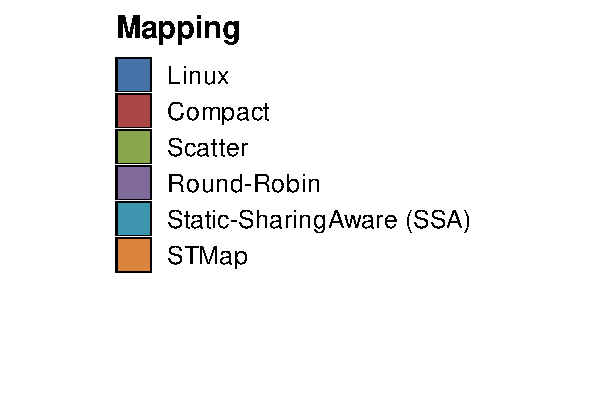
\includegraphics[width=\oneTPage\textwidth]{figures/sharingAwareThreadMapping/online/legend.pdf}}
	\caption{Execution time results on the Xeon machine.}
	\label{fig:ResultsOnlineXeon}
\end{figure}

\emph{Genome} has little contention and spends lots of time inside transactions~\cite{STAMP}. It accesses a large number of distinct addresses, roughly twice the $da\_threshold$ metric (Section~\ref{sec:calculatemap}). Since it has little contention, i.e, the abort ratio is low, the online mechanism was disabled correctly. Although there is a large difference between SSA and STMap, Scatter performed better. Looking at 96 threads SSA had a performance loss of 26\% whereas in STMap we can reduce this loss to 7.1\%, by disabling the mechanism.

\emph{Intruder} has high contention and spends medium time inside transactions~\cite{STAMP}. Results with 32 threads were similar for Compact and SSA. The performance gain achieved with STMap was 25\% in this configuration. However, as the number of threads grows, the advantages of a sharing-aware mechanism diminish. With 64 threads the performance gains were still the best, followed by Linux, but with 96 threads we had a performance loss of 16\%. This indicates that \emph{Intruder} has a sharing pattern that is strongly related to the number of threads.

\emph{Kmeans} has little contention and spends little time inside transactions \cite{STAMP}. Due to the low contention, we can expect similar results as in \emph{Genome}. However, this application accesses a very small amount of distinct addresses (roughly 20), and all accesses are made to these addresses. This shows that we cannot rely only on commit and abort ratios to predict if the application is suitable for a sharing-aware thread mapping. Using 64 and 96 threads we achieved good results with STMap, with performance gains of 30.3\% and 21.5\%, respectively. Also, it is worth noting that with 96 threads our results were even better than the SSA mechanism. This can be explained because the application has a different sharing pattern on each execution. Thus, only an online mechanism can adapt to this behavior. In 32 threads SSA achieved performance gains of 58.3\%. Hence, we expected similar results with STMap. However, we noticed an issue with the mapping interval of 100,000 used on this machine. Only in the case of 32 threads, this mapping interval was too high, and the application never triggered the mechanism. 

\emph{Labyrinth} has high contention and spends lots of time inside transactions~\cite{STAMP}. However, it accesses a large number of distinct addresses and the mechanism was correctly disabled here. Using the SSA approach we had a performance loss of 53.5\% with 32 threads. However, the STMap mechanism performed similar to Linux, in all configurations. Also, it is worth noting that all mappings performed similarly, except Compact and SSA. This application shows the importance of having a heuristic to disable the mechanism, if the mechanism can predict that the final performance would be worse.

\emph{Ssca2} has little contention, spending little time inside transactions \cite{STAMP}. The best mapping was SSA in all configurations. This application has similar characteristics as \emph{Genome}, hence, the mechanism was disabled and the results achieved with STMap were similar to Linux.

% This application needs a deeper analysis to identify other characteristics to improve the Equation~\ref{eq:enableMap}, because the mechanism was incorrectly disabled here.

\emph{Vacation} has medium contention and spends lots of time inside transactions~\cite{STAMP}. This application has complex characteristics that are harder to predict in all thread configurations. We have three distinct cases. Using 32 threads, SSA had performance gains of 5.2\% over Linux. However, due to the overhead of the mechanism, STMap was similar to Linux. Using 64 threads, the abort and commit ratio was not deterministic. We had roughly half of the times the mechanism disabled, due to a higher commit ratio. However, it is possible to see in the error bar, that sometimes the mechanism was enabled, and performed better than SSA. In 96 threads, the mechanism was incorrectly disabled all the time.

\emph{Yada} has medium contention and spends lots of time inside transactions~\cite{STAMP}. It accesses a medium amount of distinct addresses. The results in all configurations of threads were similar, with Compact and SSA performing better than other mappings. STMap performed better than Linux in all thread configurations, with performance gains of 47.1\%, 12.7\%, and 48.2\%, respectively.

\emph{Redblacktree}'s threads communicate often with their neighbors. Thus, Compact has a good performance, but when using 96 threads, STMap had the highest performance gain (58\%) over Linux.

\emph{Hashmap} has a communication pattern similar to \emph{Redblacktree}, but STMap did not result in the highest gains using 32 and 64 threads. Specifically with 64 threads, in some runs the $da\_threshold$ was higher, and since the commit ratio of this application is high, the mechanism was disabled (Algorithm~\ref{alg:enableMappig}). The execution time varies between 19 (mechanism enabled) to 71 seconds. This explains the large error bar. However, using 96 threads the mechanism was enabled in all executions, achieving performance gains of 77.7\% over Linux. %In this application, under 96 threads, the MI of 50,000 not work as expected, sometimes incorrectly disabling the mechanism.

\subsection{Results on the Opteron Machine}

\figurename~\ref{fig:ResultsOnlineOpteron} shows the performance results on Opteron. Since we already discussed the characteristics of the benchmarks in the previous section, we will only discuss the performance results.

\begin{figure}[!tb]
	\centering
	\subfigure{
		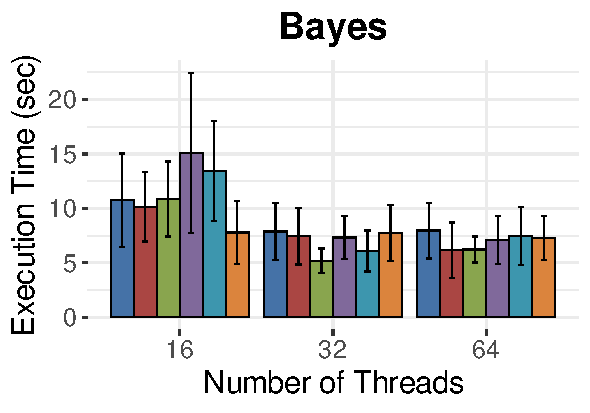
\includegraphics[width=\oneTPage\textwidth]{figures/sharingAwareThreadMapping/online/opteron/Bayes_time.pdf}
	}
	\subfigure{
		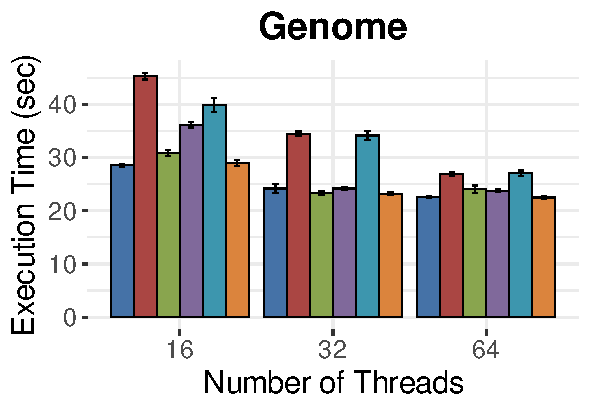
\includegraphics[width=\oneTPage\textwidth]{figures/sharingAwareThreadMapping/online/opteron/Genome_time.pdf}
	}
	\subfigure{
		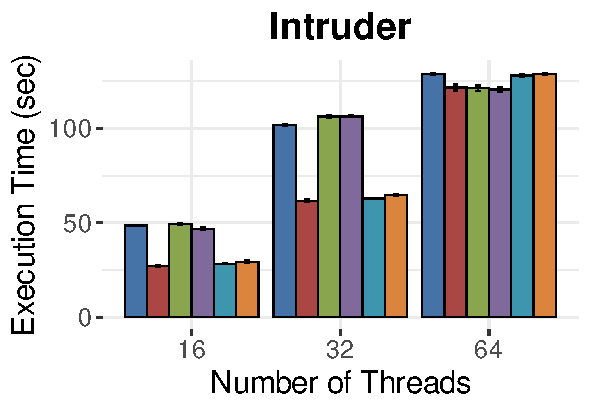
\includegraphics[width=\oneTPage\textwidth]{figures/sharingAwareThreadMapping/online/opteron/Intruder_time.pdf}
	}
	\\
	\subfigure{
		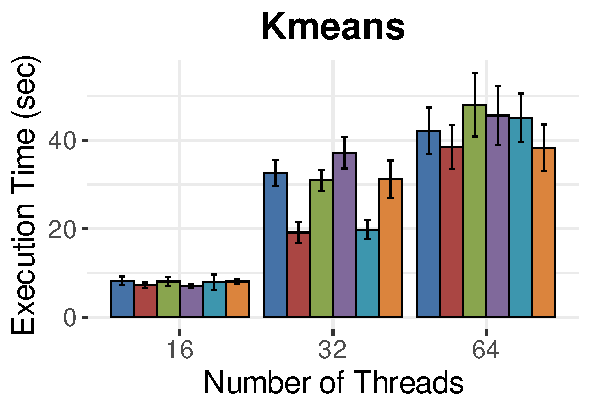
\includegraphics[width=\oneTPage\textwidth]{figures/sharingAwareThreadMapping/online/opteron/Kmeans_time.pdf}
	}
	\subfigure{
		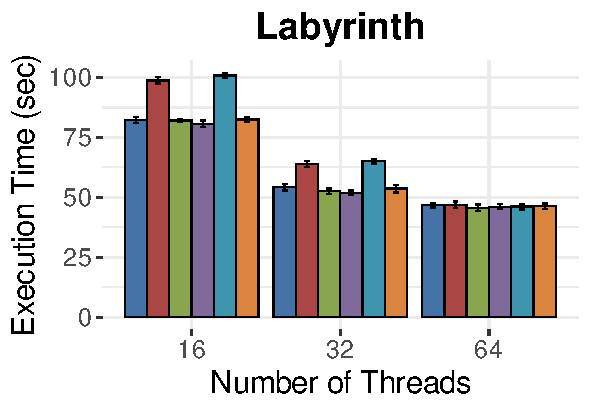
\includegraphics[width=\oneTPage\textwidth]{figures/sharingAwareThreadMapping/online/opteron/Labyrinth_time.pdf}
	}
	\subfigure{
		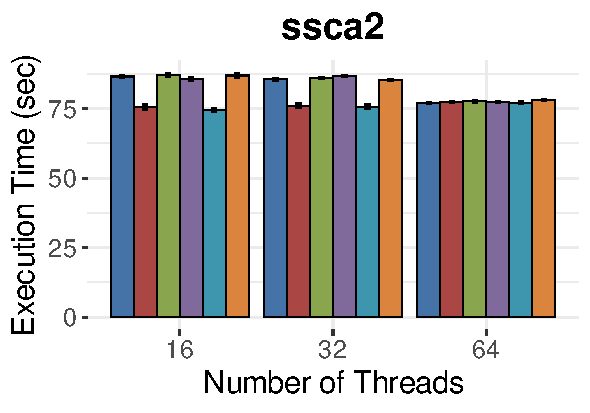
\includegraphics[width=\oneTPage\textwidth]{figures/sharingAwareThreadMapping/online/opteron/ssca2_time.pdf}
	}
	\\
	\subfigure{
		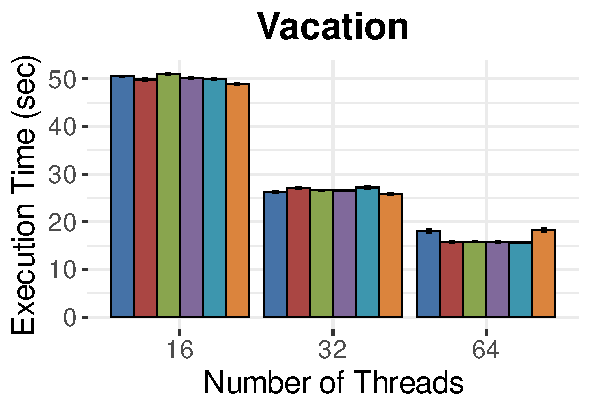
\includegraphics[width=\oneTPage\textwidth]{figures/sharingAwareThreadMapping/online/opteron/Vacation_time.pdf}
	}
	\subfigure{
		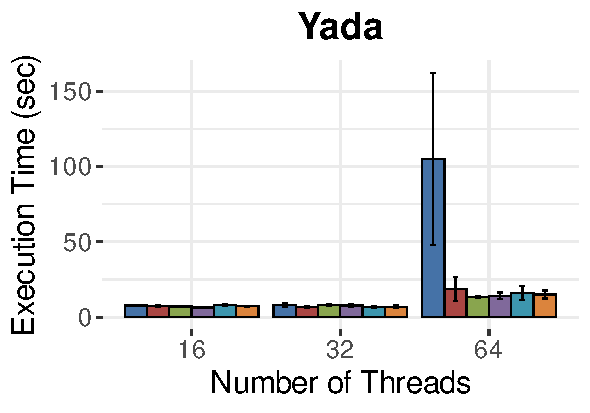
\includegraphics[width=\oneTPage\textwidth]{figures/sharingAwareThreadMapping/online/opteron/Yada_time.pdf}
	}
	\subfigure{
		\includegraphics[width=\oneTPage\textwidth]{figures/sharingAwareThreadMapping/online/opteron/Redblacktree_time.pdf}
	}
	\\
	\subfigure{
		\includegraphics[width=\oneTPage\textwidth]{figures/sharingAwareThreadMapping/online/opteron/Hashmap_time.pdf}
	}
	\subfigure {
		\includegraphics[width=\oneTPage\textwidth]{figures/sharingAwareThreadMapping/online/legend.pdf}}
	\caption{Execution time results on the Opteron Machine.}
	\label{fig:ResultsOnlineOpteron}
\end{figure}

\emph{Genome} had a similar behavior as on the Xeon machine, and STMap was disabled correctly. Using SSA, we had a performance loss with 32 and 64 threads. With 64 threads, STMap achieved the best results, roughly equal to Linux.


In \emph{Intruder} the results were similar for Compact and SSA, both for 32 and 64 threads. Nevertheless, the performance gain achieved with STMap with 16 threads was one of the best for the Opteron machine (39.4\%). Using 32 threads, the performance gains were 36.4\% compared to Linux.


In \emph{Kmeans}, contrary to the Xeon machine, the STMap mechanism was not disabled and the performance gain achieved was up to 9,1\% in 64 threads. %However, under 32 threads the gains were higher using a MI of 50,000 achieving a speedup of 38.7\%.


In \emph{Labyrinth}, the behavior was similar to Xeon. Since it accesses a large number of distinct addresses and the commit ratio is higher, the mechanism was correctly disabled. SSA resulted in performance losses, mainly with 16 and 32 threads. On the other hand, the STMap mechanism performed similarly to Linux.


\emph{Ssca2} is another application with similar behavior on both machines. Unfortunately, since the best mapping was SSA we expected good results with STMap as well. However, as on the Xeon machine, STMap was incorrectly disabled for this application.


\emph{Vacation} accesses a  large number of distinct addresses and the abort ratio was slightly greater than the commit ratio in this machine. Thus, the mechanism was correctly disabled. However, no mapping had a big impact on the performance.


\emph{Yada} accesses a medium number of distinct addresses (roughly 2,000). However, contrary to the Xeon machine, we did not observe big differences between the mappings, with exception of Linux with 64 threads. Nevertheless, SSA and STMap had similar results as Linux.


In the last two benchmarks, \emph{Hashmap} and \emph{Redblacktree}, SSA was the best mapping. STMap had slightly smaller gains compared to SSA that can be explained by the overhead in performing the mapping online.

\subsection{Discussion}\label{sect:OnlineDiscussion}

As expected, creating a unique heuristic that fits in all cases is a challenge. The main drawback of the proposed STMap mechanism appeared with \emph{Ssca2}. On both machines, STMap was disabled by the heuristic, but we had good results using the SSA approach. On the other hand, in \emph{Genome} and \emph{Labyrinth} the mechanism was correctly disabled, avoiding a greater performance loss if the mechanism was enabled. Analyzing the results, sharing-aware thread mapping in STM depends on a low number of distinct addresses with a lot of accesses in these addresses. Also, applications with low and medium contention had higher gains.

Prior work on sharing-aware mapping focused solely on analyzing the communication matrix to detect if applications would benefit from a new thread mapping \cite{Diener2015,Bordage:2018}. However, our proposal to perform online sharing-aware thread mapping  inside STM applications is based on the distinct addresses, commit, and abort ratios and proved to be accurate.

On the Opteron machine, the highest performance gain over Linux was achieved by \emph{Yada} using 64 threads (85.8\%) and by Intruder using 16 threads (39.4\%). On the Xeon machine, the highest performance gain was achieved by \emph{Hashmap}, achieving gains of 77.7\% over Linux. %Finally, using a mapping interval of 100,000 presented higher gain on both machines.
%\blue{Taking into consideration all applications and thread configurations, STMap achieved the best average speedup on the Opteron machine (9.1\%) compared to Linux, followed by Compact (7.9\%). On the Xeon machine, SSA achieved the best average speedup (22.3\%) followed by STMap (17.6\%).}
To summarize, \tablename~\ref{tab:resultsOnline} shows the average performance gains of each mechanism over Linux, taking into consideration all applications and thread configurations.
\begin{table}[tb]
	\centering
	\caption{Average performance gains of each mechanism over Linux.}
	\label{tab:resultsOnline}
	\begin{tabular}{lrrrrr}
		\toprule
		\textbf{Machine}  & \textbf{Compact} & \textbf{Scatter} & \textbf{Round\textbf{}Robin} & \textbf{SSA} &  \textbf{STMap} \\
		\midrule
		\textbf{Xeon}   & 15.88\%          & 13.14\%          & 14.50\%            & 22.32\%   &  19.07\%        \\
		\textbf{Opteron} & 7.96\%           & 5.86\%           & 3.15\%            & 6.50\%     & 9.78\%       \\
		\bottomrule
	\end{tabular}
\end{table}

\subsection{Mechanism sensitivity}\label{sec:sensitivity}

The STMap performance improvements are sensitivity to the mapping interval used in the heuristic to trigger the mechanism (Algorithm~\ref{alg:commAndMap}). We execute additional experiments varying the mapping interval, between 25,000 to 200,000 to verify if the chosen mapping interval of 100,000 was in fact the best one for the two machines. \figurename~\ref{fig:sensitivity} shows the performance gains achieved with each mapping interval, grouped by machine.

\begin{figure}[!ht]
	\centering
	\includegraphics[width=0.8\textwidth]{figures/sharingAwareThreadMapping/sensitivity/sensitivity.pdf}
	\caption{Mechanism sensitivity when changing the mapping interval.}
	\label{fig:sensitivity}
\end{figure}

The results confirm that a mapping interval of 100,000 presents the best overall results on both machines. The mapping interval of 200,000 does not present good results because the majority of the applications do not access these quantity of addresses in one thread. Hence, for these applications the mechanism was never triggered, because the mapping interval was never reached. Although a mapping interval of 25,000 in the Xeon machine presents, on average, good results, some observations are necessary. We choose 2 applications for this discussion. \figurename~\ref{fig:ResultsSensitivyXeon} compares the results of STMap using the best mapping interval of 100,000 to the mapping interval of 25,000.


\begin{figure}[ht]
	\centering
	\subfigure{
		\includegraphics[width=\oneTPage\textwidth]{figures/sharingAwareThreadMapping/sensitivity/Genome_time.pdf}
	}%
	\subfigure{
		\includegraphics[width=\oneTPage\textwidth]{figures/sharingAwareThreadMapping/sensitivity/ssca2_time.pdf}
	}%
	\subfigure{
		\includegraphics[width=\oneTPage\textwidth]{figures/sharingAwareThreadMapping/sensitivity/legend.pdf}
	}%
	\caption{Comparing STMap using different mapping intervals on the Xeon machine.}
	\label{fig:ResultsSensitivyXeon}
\end{figure}

As mentioned in Section~\ref{sec:calculatemap}, \emph{Genome} is an application that is not suitable for a sharing-aware thread mapping. Hence, it is necessary to disable the mechanism to not hurt the performance. However, as shown in \figurename~\ref{fig:ResultsSensitivyXeon}, using a mapping interval of 25,000 the mechanism was enabled. However, it was not deterministic, with sometimes the mechanism being disabled, as shown in the large errors bars. We see similar non-determinism in \emph{Ssca2}. As mentioned in Section~\ref{sect:OnlineDiscussion}, \emph{Ssca2} was the main drawback of the mechanism in the mapping interval of 100,000. Nevertheless, on average, in \emph{Ssca2} the results of the mapping interval of 25,000 were better, helping to decrease the average execution time of the mechanism using 25,000.

\section{Summary}

This chapter presented two mechanisms to perform sharing-aware thread mapping for STM applications. Although only transactional operations are tracked to extract the memory access behavior, the experimental results of the \emph{Static-SharingAware}~(SSA) mechanism shown that only the information inside the transactional memory system is enough to improve the performance of STM applications.

The next proposed mechanism, \emph{STMap}, which is an online mechanism to extract the memory access behavior of STM applications and use this information to calculate a sharing-aware mapping of threads to cores. The main advantage is that no prior knowledge is necessary, all phases are executed while the application is running. Also, applications are not modified, only the STM system. Although we only trigger thread mapping one time, since the used applications do not present dynamic sharing behavior, we believe that the mechanism can work for a wide range of STM applications since (1) the chose sampling interval of 100 represents a very small overhead to the final execution time and (2) if the mechanism was not disabled, the next trigger time would in the mapping interval of 200,000. However, the experiments made on the mechanism sensitivity (Section~\ref{sec:sensitivity}) showed that the majority of the applications do not access these quantities of addresses in one thread.

Overall, both mechanisms showed performance gains when compared to other static thread mapping strategies and the default Linux CFS scheduler.
